\documentclass{article}

\usepackage{repsty}
\usepackage{wrapfig}

\usepgfplotslibrary{fillbetween}

\newcommand{\dt}{\Delta t}
\newcommand{\dtm}{\dt_{\meas}}
\newcommand{\dtc}{\dt_{\cnt}}
\newcommand{\LTb}{\tau_b}
\newcommand{\lamb}{\lambda_b}
\newcommand{\pdet}{p}
\newcommand{\pscat}{p_s}

\begin{document}
	
		
\section*{Preliminary}

The beam current falls according to the B-L law:
\[
	I(t) \equiv N^b(t)\nu = I_0\cdot e^{\lamb t}.
\]

A fraction $p$ of the beam particles will be scattered in the direction of the detector; in time $\dtm$, the number of particles collected at the detector will be
\begin{align}
	N_0(t) & = p\cdot\int_{-\dtc/2}^{+\dtc/2} I(t+\tau)\td\tau \notag                    \\
	       & = p\cdot\frac{\nu N_0^b}{\lamb} e^{\lamb t}\cdot \bkt{e^{\lamb\sfrac{\dtc}{2}} - e^{-\lamb\sfrac{\dtc}{2}}} \notag \\
	       & \approx \underbrace{p\cdot\nu N_0^b e^{\lamb t}}_{\text{rate}~r(t)} \cdot\dtc.~\footnotemark
\end{align}
\footnotetext{Average number of events in a time interval is rate times interval:~\cite{CountRateStat}.}

This is on average. To model the actual number, the Poisson distribution will be appropriate:
\[
	P_{N_0(t)}(\tilde{N}_0) = \frac{\bkt{r(t)\dtc}^{\tilde{N}_0}}{\tilde{N}_0!}\cdot e^{-r(t)\dtc}.
\]
The variance is equal to the mean: $\SD{\tilde{N}_0}^2(t) = N_0(t)$. In the limit of large $N_0(t)$, the Poisson distribution becomes Gaussian.

$\tilde{N}_0$ is what we actually measure in $\dtc$. To estimate the expectation $N_0(t)$ (and its variance), we have to take the mean (variance) of the Gaussian. For that we take several measurements, and estimate the parameters as usual, i.e. as sums of random variables, i.e. distributed normally. The number of measurements we can make during $\dtm$ is $\Ncm = \dtm/\dtc$. The standard error of the mean then is 
\begin{align}\label{eq:MeasSE}
	\SD{N_0}(t) & = \SD{\tilde{N}_0}(t)/\sqrt{\Ncm} = \sqrt{N_0(t)\frac{\dtc}{\dtm}}            \notag \\
	            & \approx \sqrt{\frac{p\cdot\nu N_0^b}{\dtm}}\cdot\dtc \cdot\exp\bkt{\frac{\lamb}{2}\cdot t}.
\end{align}
\newcommand{\A}{\frac{1}{\sqrt{p\cdot\nu N_0^b}}}

Relative error,
\[
	\frac{\SD{N_0}(t)}{N_0(t)} \approx \frac{A}{\sqrt{\dtm}}\cdot\exp\bkt{-\frac{\lamb}{2}t} = \frac{A}{\sqrt{\dtm}}\cdot\exp\bkt{\frac{t}{2\LTb}},~ A=\A,
\]
grows.

\section{Problem statement}
Define the following variables: \begin{inparaenum}[\itshape a\upshape)]
	\item the number of measurements per node: $\Nmnd$,
	\item the number of nodes per experiment: $\Nnd$.
\end{inparaenum}

We have to fit the function
\begin{equation}\label{eq:Signal}
N(t) = N_0(t)\cdot\bkt{1 + P\cdot e^{-\sfrac{t}{\tau_d}}\cdot\sin(\omega\cdot t + \phi)},
\end{equation}
given $\Nm = \Nnd\cdot\Nmnd$ sample points.

Assuming the Gaussian error distribution with mean zero and variance $\nu \equiv \SD{\meas}^2 = \SD{N_0}^2(t)$, the maximum likelihood estimator for the variance of the frequency estimate can be expressed as
\begin{align*}
\var{\hat\omega} &= \frac{\nu}{X_{tot}\cdot \var[w]{t}}, \\
X_{tot} &= \sum_{j=1}^{\Nm} x_j = \sum_{s=1}^{\Nnd}\sum_{j=1}^{\Nmnd} x_{js}, \\
\var[w]{t} &= \sum_i w_i \bkt{t_i - \avg{t}_w}^2,~ \avg{t}_w = \sum_i t_i w_i, \\
w_i &= \frac{x_i}{\sum_j x_j},~ x_i = (N_0P\exp(\lambda t_i))^2\cos^2(\omega t_i + \phi) = \bkt{\mupp}^2.
\end{align*}

The three factors, contributing to the standard error of the estimate are:
\begin{inparaenum}[\itshape a\upshape)]
	\item the error variance $\nu = \SD{N_0}(t)^2$ (governed by the number $\Ncm$ of polarimetry measurements per signal measurement~\eqref{eq:MeasSE}), 
	\item the time spread $\sum_i w_i (t_i - \avg{t}_w)^2$ of the sample measurements, and
	\item their net informational content $X_{tot}$.
\end{inparaenum}


\section{Informational content}
\DeclareDocumentCommand{\stat}{s}{\IfBooleanTF{#1}{X_{tot}}{\frac{\SD{\meas}^2}{\SE{\hat\omega}^2\cdot \var[w]{t}}}}
\newcommand{\dtnd}{\dt_{zc}}

We can express $\sum_{j=1}^{\Nmnd} x_{js} = \Nmnd \cdot x_{0s}$, for some mean value $x_{0s}$ in the given node $s$. The sum $\sum_{j=1}^{\Nmnd} x_{js}$ falls exponentially due to decoherence, hence $x_{0s} = x_{01}\exp{(\lambda\cdot \frac{(s-1)\cdot\pi}{\omega})}$. Therefore,
\begin{align}
	X_{tot} & = \Nmnd\cdot x_{01} \cdot \frac{\exp{\bkt{\frac{\lambda\pi}{\omega}\Nnd}}-1}{\exp{\bkt{\frac{\lambda\pi}{\omega}}}-1} 
	\equiv \Nmnd \cdot x_{01}\cdot g(\Nnd); \label{eq:FItot}\\
	x_{01}  & = \frac{1}{\dtnd}\int_{-\dtnd/2}^{+\dt/2}\cos^2(\omega\cdot t)\td t = \frac12\cdot \bkt{1 + \frac{\sin\omega\dtnd}{\omega\dtnd}},                                    \label{eq:MeanFIZC}   \\
	\Nmnd   & = \frac{\dtnd}{\dtm}. \label{eq:NumMeasNode}
\end{align}

Eq.~\eqref{eq:FItot} can be used to estimate the reasonable experiment duration. $g(\Nnd)$ is a limited function; in Figure~\ref{fig:GofT} it is shown for different life-times. In Table~\ref{tbl:FItot} we have the time (in signal life-times) required to reach the different levels of information; the signal-to-noise ratios there are computed under the assumption of constant relative error.
\begin{figure}[h]
	\centering
	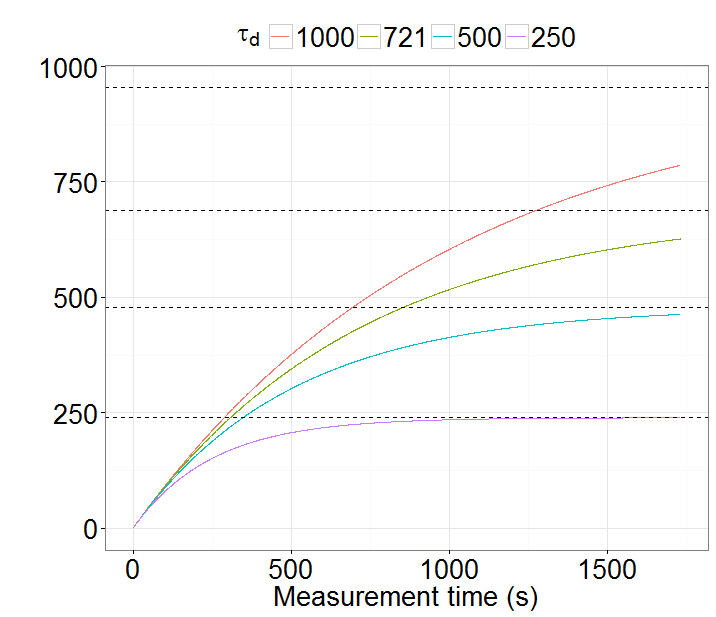
\includegraphics[scale=.5]{../MEPhI/img/XtotOnTime}
	\caption{$[g\circ t](\Nnd)$ for different life-times $\tau = \sfrac1\lambda$.\label{fig:GofT}}
\end{figure}
\begin{table}[h]
	\centering
	\caption{Total Fisher information table\label{tbl:FItot}}
	\begin{tabular}{rrr}
		\hline
		FI limit (\%) & Reached ($\times\tau$) & SNR@3 \%error \\ \hline
		95 &                    3.0 &            1.7 \\
		90 &                    2.3 &            3.3 \\
		70 &                    1.2 &           10.0 \\
		50 &                    0.7 &           16.5 \\
		\hline
	\end{tabular}
\end{table}

Eq.~\eqref{eq:MeanFIZC}, together with eq.~\eqref{eq:NumMeasNode} and
\[
	\stat* = \stat,
\]
produce an equation by which the required compaction time $\dtnd$ can be found:
\begin{equation}
	\dtnd + \frac{\sin\omega\dtnd}{\omega} - 2\cdot \stat* \cdot\dtm \cdot g(\Nnd)^{-1}= 0.
\end{equation}

\begin{figure}[h]
	\centering
	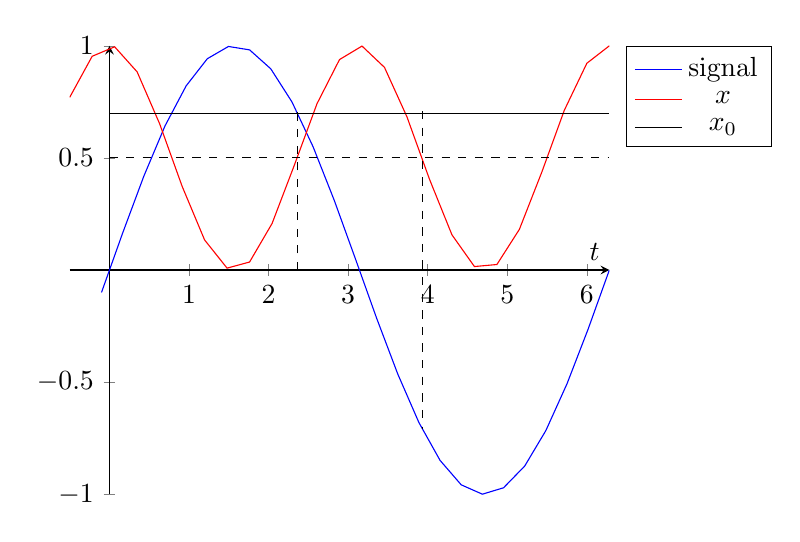
\begin{tikzpicture}
	\begin{axis}[axis lines=center, xlabel=$t$, domain=-.5:2*pi, legend pos=outer north east]
	\addplot[color=blue, name path=signal, domain=-.1:2*pi] {sin(deg(x))}; \addlegendentry{signal}
	\addplot[color=red] {cos(deg(x))^2}; \addlegendentry{$x$}
	\addplot[mark=none, domain=0:2*pi]{.7}; \addlegendentry{$x_0$}
	\addplot[mark=none,dashed, domain=0:2*pi]{.5};
	\draw[dashed] (axis cs:2.36,0) -- (axis cs:2.36,{sin(deg(2.36))});
	\draw[dashed] (axis cs:3.93,{-sin(deg(3.93))}) -- (axis cs:3.93,{sin(deg(3.93))});
	\end{axis}
	\end{tikzpicture}
	\caption{Explanation for $x_0$\label{fig:x0Expl}.}
\end{figure}

\pagebreak

\begin{align*}
	X_{tot}	&= \Nmnd\cdot \tilde{g}(\Nnd)\cdot x_{01}, \\
	X_{tot}	&= \stat
\end{align*}

\begin{align}\label{eq:CmpTimeEq}
 \notag
\end{align}

The factor $\stat*$ reflects the amount of necessary Fisher information to reach the required statistical precision. The less the ratio $\SE{\hat{\omega}}/\SD{\meas}$, the more information is required. That information requirement can be fulfilled in two ways: via the increase in the number of nodes (total time), or the increase of the compaction time. The gain in information provided by the former is limited by the term $\tilde{g}(\Nnd)$ due to decoherence. Because of it, the compaction factor in my simulation is $\approx 1$ (i.e. no sense in modulation), for the ratio $\approx 1$, and total measurement time $\approx 2.4\tau_d$. For even less ratios, there doesn't even exist a solution for~\eqref{eq:CmpTimeEq}. That is, because of the decoherence, even if we collect the data uniformly in time (with frequency 5000 measurements per second), we won't have enough information to estimate $\omega$ with the required precision.



\begin{thebibliography}{9}
	\bibitem{CountRateStat}
	\url{http://www.owlnet.rice.edu/~dodds/Files331/stat_notes.pdf}.
\end{thebibliography}

\end{document}